%\documentclass[11pt,twoside,lineno]{GSA_format}
\documentclass[10pt,twoside, twocolumn]{GSA_format}
% Use the documentclass option 'lineno' to view line numbers
\usepackage[normalem]{ulem}
\usepackage{float}
\usepackage{amsmath,amssymb}
%\usepackage[textwidth=25cm]{geometry}
\usepackage{siunitx}
\usepackage{arydshln}
\usepackage{graphicx}

\useunder{\uline}{\ul}{}
\articletype{inv} % article type

\newcommand{\bm}[1]{\mbox{\boldmath{$#1$}}}

\newcommand{\beginsupplement}{%
        \setcounter{table}{0}
        \renewcommand{\thetable}{S\arabic{table}}%
        \setcounter{figure}{0}
        \renewcommand{\thefigure}{S\arabic{figure}}%
     }
     
\title{Background selection under evolving recombination rates}

\author[$\ast$]{Tom R. Booker}

\affil[$\ast$]{Department of Zoology, University of British Columbia}

\keywords{Evolutionary genetics, recombination rate, background selection}

\runningtitle{Background selection and recombination rate evolution} % For use in the footer 

\runningauthor{Booker et al}

\begin{abstract}

Background selection (BGS), the effect that purifying selection exerts on evolution at linked sites, is expected to be ubiquitous across eukaryotic genomes. BGS effects reflect the interplay of fitness effects and rates of deleterious mutations with the recombination rate.  Leveraging the theory of BGS to analyse patterns of nucleotide diversity has shed light on central issues in evolutionary biology. Fundamental to theoretical models of BGS are recombination rate estimates and an assumption that recombination rates are invariant over time. However, in some lineages recombination rates evolve very rapidly violating this central assumption. Here, we investigate the effect that recombination rate evolution can have on BGS. We show that recombination rate evolution may have localised effects and cause analyses to underestimate the effects genome-wide effects of BGS. Indeed, we find evidence that rapid recombination rate evolution in the recent history of the house mouse may impact inferences of selection in that species.

%It is expected that background selection (BGS), the effect that purifying selection exerts on evolution at linked sites, is ubiquitous across eukaryotic genomes.  The effects of BGS reflect the interplay of the fitness effects and rate of deleterious mutations with the recombination rate.  Leveraging the theory of BGS to analyse patterns of nucleotide diversity in various lineages has shed light on central issues in evolutionary biology. Fundamental to theoretical models of BGS are recombination rate estimates and an assumption that recombination rates are invariant over time. However, in some lineages recombination rates evolve very rapidly violating this central assumption. In this short report, we investigate the effect that recombination rate evolution can have on BGS. We show that recombination rate evolution has an effect on BGS that resembles the effects of population size change. Unlike population size change, however, which may affect the entire genome, recombination rate evolution may have localised effects cause analyses to underestimate the effects genome-wide effects of BGS and demonstrate. Indeed, we find evidence that rapid recombination rate evolution in the recent history of the house mouse may impact inferences of BGS and other forms of selection in that species.

\end{abstract}

\begin{document}

\maketitle

\marginmark

\firstpagefootnote


\correspondingauthoraffiliation{1}{Corresponding author: booker@zoology.ubc.ca}
\vspace{-33pt}% Only used for adjusting extra space in the left column of the first page

\section{Introduction}

Different modes of selection (e.g. positive, purifying and balancing) can all affect variation at linked sites (reviewed in Charlesworth 2008). In the case of purifying selection, the removal of deleterious mutations  can cause linked neutral variants to be lost along with them through a process referred to as background selection (BGS; Charlesworth et al 1993). Of the mutations that affect fitness, the vast majority are likely deleterious with a comparatively small proportion of beneficial mutations (Keightley and Eyre-Walker review). For those reasons, it has been proposed that BGS is likely ubiquitous across eukaryotic genomes and should be incorporated into the null model for molecular evolution (Comeron 2014; Gilbert and Pouyet 2020; Jensen et al 2018; Johri et al 2020).

% providing evolutionary biologists with a framework for understanding natural selection through the analysis of genome-wide patterns of nucleotide diversity.  \\
\vspace{5px}

One effect of BGS is a reduction in genetic diversity for regions of the genome subject to purifying selection. The expected reduction in nucleotide diversity ($\pi$) under BGS is proportional to the ratio of the local deleterious mutation rate and the local recombination rate (Charlesworth et al 1993; Nordborg 1996; Hudson and Kaplan 1995). The first empirical evidence that selection at linked sites of any kind influences genetic variation across the genome came from studies in \textit{Drosophila}. Aguad\'e et al (1989) measured genetic variability in the \textit{yellow-achaete-scute} regions located at the tip of the X-chromosome in \textit{D. melanogaster}. The \textit{yellow-achaete-scute} regions experience restricted crossing-over and Aguad\'e et al (1989) found that they harbour far less genetic variation than had been reported for more highly recombining regions of the genome. Subsequent studies demonstrated a positive correlation between nucleotide diversity and recombination rate genome-wide in \textit{D. melanogaster} (Begun and Aquadro 1993; Andolfatto 2002) and similar patterns have been reported in numerous other species (Cutter and Payseur 2012). 

\vspace{5px}

Interpreting genome-wide patterns of genetic variability in terms of selection at linked sites requires accurate estimates of population genetic parameters. Empirical estimates of the recombination rate can be obtained by examining the inheritance of genetic markers through known pedigrees, as in traditional genetic mapping, or by directly comparing an individual's genome to that of its gametes (e.g. Sun et al 2019). Both methods directly observe recombination events over one or fairly small number of generations, and thus provide recombination rate estimates for contemporary populations. Alternatively, recombination rate estimates can be obtained indirectly by analysing linkage disequilibrium across the genome (REFs) and such estimates reflect both recent and ancestral recombination events. The use of empirical or indirect estimates of recombination rate when analysing genome-wide variation in $\pi$ in terms of BGS implicitly assumes that recombination rates have not changed over the time in which patterns of diversity have been established under BGS.

\vspace{5px}

However, recombination rate landscapes can evolve rapidly. For example, there has been extensive evolution of recombination rates at broad and fine scales in the house mouse (\textit{Mus musculus}). Due to the requirement of at least one cross-over per chromosome per meiosis in mammals, karyotype evolution likely influences recombination rate landscapes at broad scales. The lineage leading to \textit{M. musculus}  (2\textit{n}=40) has experienced large chromosomal rearrangements since it shared a common ancestor with \textit{Mus pahari} (2\textit{n}=48) 5 million years ago (Thybert et al 2018). Moreover, there are differences in recombination rate among populations of \textit{Mus musculus domesticus} that harbour different karyotypes (Vara et al 2021). Recombination events in mice are typically restricted to narrow windows of the genome (on the order of 5-10 Kbp), referred to as hotspots (Paigen et al 2007). The locations of recombination hotspots in mice, as well as humans and many other vertebrates, are determined by the binding of a protein encoded by the \textit{PRDM9} gene to specific DNA motifs (Baudat et al 2010; Baker et al 2017). There is evidence that \textit{PRDM9} has undergone recurrent bouts of positive selection in mice (Oliver et al 2009) and natural populations of \textit{M. musculus spp.} harbour various \textit{PRDM9} alleles corresponding to different suites of recombination hotspots  (Smagulova et al 2015). Overall, there is clear evidence that recombination rates have evolved at broad and fine scales in mice in the relatively recent past. 

\vspace{5px}

Recombination rate changes may influence fine-scale patterns of molecular evolution. For example, chromosomal fusions would decrease recombination rates experienced by individual nucleotides, and thus increase the effects of BGS and other processes mediated by recombination. Consistent with this, Cicconardi et al (2021) found evidence suggesting that chromosomes that underwent fusions in the ancestors of extant \textit{Heliconius} butterfly species now harbour lower $\pi$ due to reduced recombination rates. Following evolution of the recombination rate landscape, there will be a lag period wherein patterns of genetic variability more closely reflect ancestral recombination rates than derived rates. Depending on how recombination rate landscapes evolve, analysis of BGS in lineages that are still within that lag period may be obscured. For example, the hallmark signature of selection at linked sites, a positive correlation between nucleotide diversity and recombination rate may not be clearly observed. In this letter, we examine how patterns of neutral genetic variability under BGS respond to evolution of the recombination rate and describe how this would affect analyses that are used to identify the effects of selection genome wide. 

\section{Results and Discussion}

\subsection{Background selection under evolving recombination rates}
%The analogy is not perfect, because it does not capture the effects of weakly deleterious mutations (BGS Papers). 

A change in the recombination rate will alter the effects of BGS. When deleterious mutations have large effects on fitness, BGS resembles a localised reduction in the effective population size ($N_e$). So, changes in the recombination rate for a particular genetic region may resemble a localised change in $N_e$. Indeed, an expression that describes coalescence times after a change in population size (Equation \ref{BGS_rec}) accurately predicts the effects of BGS under recombination rate evolution (Figure \ref{fig:BGS_over_time_fixed_s}). It takes around $4N_e$ generations for nucleotide diversity to closely reflect an increase or a decrease in the recombination rate (Figure \ref{fig:BGS_over_time_fixed_s}). Up to $2N_e$ generation after such a change, however, nucleotide diversity under BGS more closely resembles the expectation under the ancestral recombination rate than it does the derived rate (Figure \ref{fig:BGS_over_time_fixed_s}). Assuming a distribution of fitness effects for harmful mutations leads to a similar result (Figure S1).

The fit of this breaks down when deleterious mutations have only mild effects on fitness (Figure X) because in such cases BGS does not resemble a simple reduction in $N_e$ (Good et al 2014; Cvijović et al 2018). 

\vspace{5px}


\begin{figure}[H]
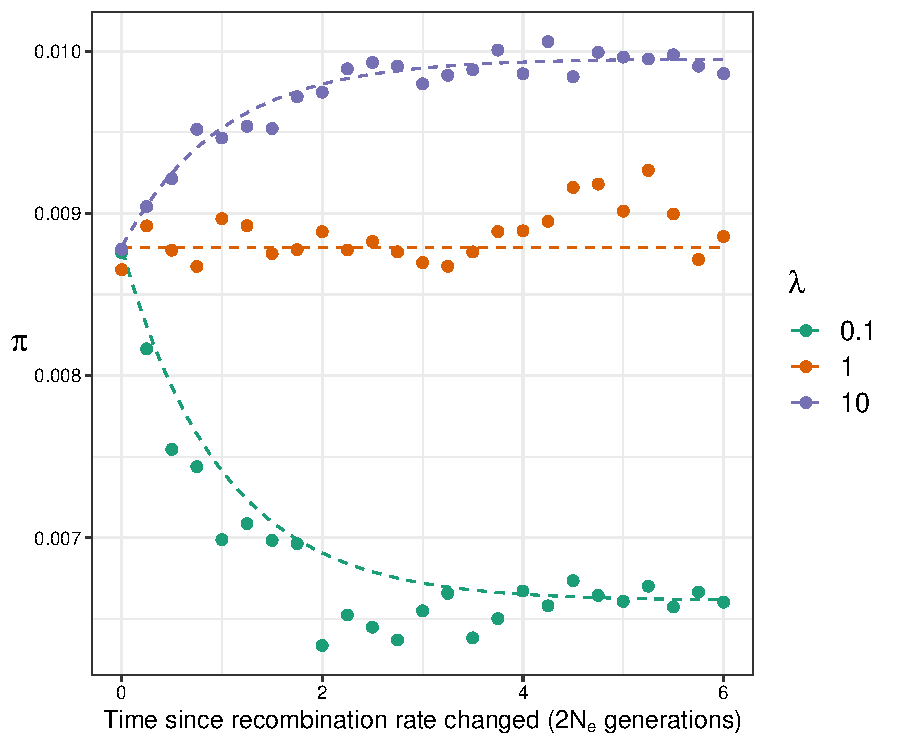
\includegraphics[width=0.5\textwidth]{../TheoreticalExpectation/B_over_time_fixed_s_plot_singlePanel}
\caption{Nucleotide diversity over time after recombination rates change by a factor $\lambda$. The dashed lines were calculated using Equation \ref{BGS_rec}, points indicate the mean from 100 replicate simulations.}
\label{fig:BGS_over_time_fixed_s}
\end{figure}

For the sake of simplicity, the model we used assumes that recombination rates evolve instantaneously. While that is obviously an oversimplication, there is reason to expect that recombination rate changes may evolve rapidly. Chromosomal fusions can exhibit meiotic drive (Chmátal et al 2014) so may spread to fixation very rapidly and there is evidence that the \textit{PRDM9} gene that controls the location of recombination hotspots in many vertebrate species has undergone recurrent bouts of positive selection (Oliver et al 2009). 

\vspace{5px}

Empirical recombination rate estimates (i.e. obtained from direct observation of recombination events) reflect contemporary populations, but indirect estimates may reflect a combination of ancestral and contemporary rates. Figure XY shows that indirect estimates recombination rates estimates obtained from patterns of LD very quickly reflect the changed (Spence et al 2018) 



\subsection{Evolving recombination rates and evidence for natural selection}

When a population is sampled during the lag period after evolution of the recombination rate (e.g. before $2N_e$ generations have elapsed), inferences made from genomic data about molecular evolution may be obscured. The  effect that recombination rate evolution will have on inferences made about molecular evolution will, of course, depend on how recombination rates change. We performed two sets of simulations to demonstrate effects of recombination rate evolution. In the first, we simulated a dramatic rearrangement of the recombination rate map at broad scales (Figure S2). In the second, we modelled fine-scale recombination rate evolution by shifting the landscape of recombination hotspots (Figure S2). 




The lineage leading to \textit{Mus musculus} underwent a bout of karyotype evolution around 3 MYA (Thybert et al 2018). Thybert et al (2018) identified ancestral chromosomal rearrangements in the lineage leading to \textit{M. musculus} using an alignment of rodent genomes. We classified \textit{M. musculus} chromosomes as either "non-conserved" or "conserved" based on whether Thybert et al (2018) identified ancestral rearrangements or not, respectively.

\vspace{5px}

We compared the correlation between $\pi$ and $r$ on the conserved and non-conserved chromosomes of \textit{Mus musculus domesticus} using previously analysed data from Kartje et al (2020)(Table \ref{Table1}). We found a pattern suggesting that $\pi$ does not fully reflect the current recombination rate regime in \textit{Mus musculus}. The correlation between $\pi$ and $r$ was weaker and less significant for the non-conserved chromosomes compared to the conserved chromosomes in all cases tested (Table \ref{Table1}). 

For Gough island mice, the correlation was  
suggests that \textit{M. musculus} has 









\begin{figure}[H]
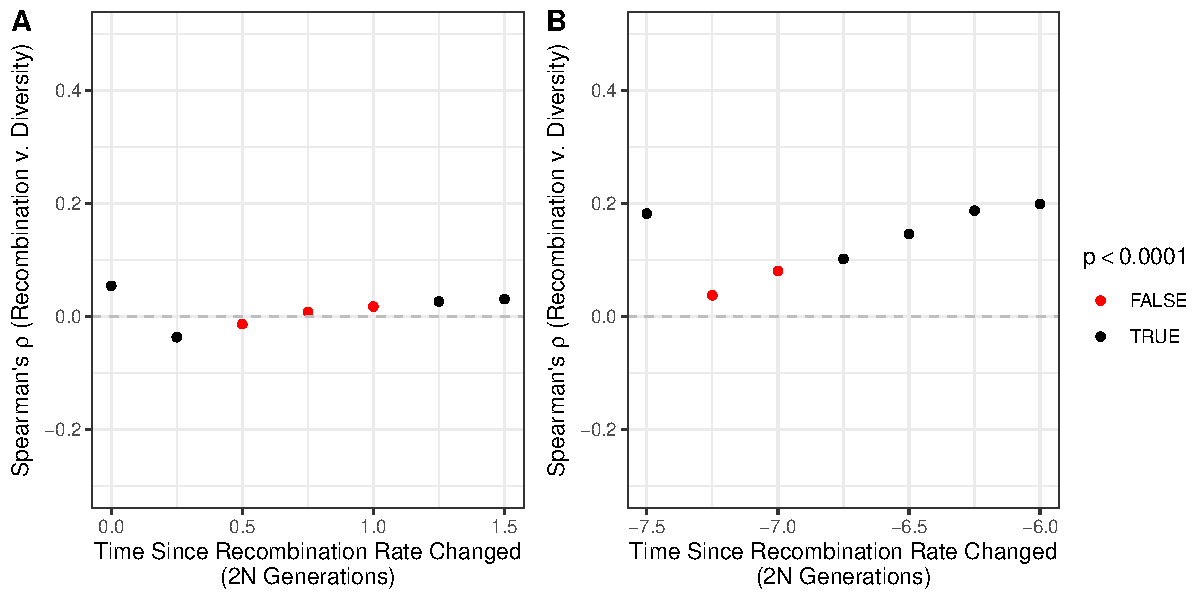
\includegraphics[ width = 0.5\textwidth]{../Plots/pi_r_correlationOverTime_bothMaps.pdf}
\caption{Spearman's correlation between nucleotide diversity ($\pi$) and recombination rate ($r$) over time after recombination rates evolve. Results are shown for 100 Kbp analysis windows. } 
\end{figure}




\begin{table*}[t]
\
\resizebox{\textwidth}{!}{\begin{tabular}{cc|
           *{2}{S[round-mode = figures,
            round-precision = 3]}|
                 *{2}{S[round-mode = figures,
            round-precision = 3]}|
                 *{2}{S[round-mode = figures,
            round-precision = 3]}}
                 \hline
 & & \multicolumn{2}{c}{Whole Genome} & \multicolumn{2}{c}{Conserved Chromosomes}& \multicolumn{2}{c}{Non-Conserved Chromosomes}\\
 {Window} & {Population} &  {Spearman`s $\rho$} & {$p$-value} &{Spearman`s $\rho$} & {$p$-value} & {Spearman`s $\rho$} & {$p$-value}\\ 
  \hline
5Kbp& Gough Island & 0.00766946556467726 & \num{4.28487483542177e-05} & 0.00879560871962056 & 0.0102132179985377 & 0.00485568404015206 & 0.0301693742321603 \\ 
  5Kbp & France & 0.00408044307052427 & 0.0294929095581957 & 0.0402631172537313 & \num{6.10313340830373e-32} & -0.0107049632666829 & \num{1.75806407865671e-06} \\ 
  5Kbp & Germany &  0.00752167382031877 & \num{6.05264156648312e-05} & 0.0151531276721775 & \num{9.6335227129151e-06} & 0.00386135398506519 & 0.0849380013628119 \\ 
  1Mbp & Gough Island &  0.0535515289545324 & 0.00946379855975982 & 0.0588327090738239 & 0.124246200526924 & 0.043697649001863 & 0.0748313470537267 \\ 
  1Mbp & France &  0.0449712235482249 & 0.0293606123894296 & 0.134981255195878 & 0.000400166310010629 & 0.00998569897732337 & 0.684066944892074 \\ 
  1Mbp & Germany &  0.0535221710805316 & 0.00953371381645413 &  0.0774668203290588 & 0.0428305229197646 & 0.0425693100291219 & 0.0828457161038532 \\ 
\hline
\end{tabular}}

\caption{The correlation between nucleotide diversity ($\pi$) and recombination rate for three populations of house mice (\textit{Mus musculus domesticus}) calculated from all autosomes, conserved chromosomes that exhibit no syntenic breaks between \textit{M. musculus} and \textit{M. pahari} and the non-conserved chromosomes as identified by Thybert et al (2018).}
\label{Table1}
\end{table*}


Numerous species that have been examined do not exhibit a positive correlation between diversity and recombination rate (Cutter and Payseur). For example, wild and domesticated rice species (\textit{Oryza rufipogon} and \textit{Oryza sativa}, respectively) exhibit negative correlations between diversity and recombination rate, potentially due to a positive correlation between functional density and recombination rate in those species (Flowers et al 2011). 

In comparison to mammals, birds have fairly conserved karyotypes and in some cases highly conserved recombination landscapes (REF; Singhal et al 2017). 



We have restricted our analysis to what happens when fitness affecting mutations are strictly deleterious and generate BGS. However, other modes of selection and their effects on linked variation may also affect nucleotide diversity. For example, there is evidence that recurrent selective sweeps influence diversity patterns in numerous species (Nam et al; Booker et al 2021; Campos et al ; Elyashiv et al ). It seems reasonable to expect that recombination rate evolution would also influence inferences about selective sweeps.  


In mice, nucleotide divergence between \textit{Peromyscus eremicus} and \textit{P. maniculartus} exhibits a clear negative correlation with chromosome size, but for \textit{Mus pahari}, sister species to \textit{M. musculus}, there is no such correlation (Tigano et al 2021). Tigano et al (2021) performed analyses that suggest that karyotype evolution caused gave rise to shifts in the contribution of ancestral diversity to divergence. 

\section{Methods}
\subsection{Model}
Background selection has been modelled as the reduction in effective population size ($N_e$) at a neutral site due to the removal of deleterious variants. The effects of background selection are often expressed as $B = \frac{N_e}{N_0}$, where $N_e$ is the effective population size and $N_0$ is the expected population size under strict neutrality. In a non-recombining genome, $B$ is proportional to the ratio of the deleterious mutation rate to the strength of selection acting on harmful mutations (Charlesworth et al 1993). For a neutral site present on a recombining chromosome, the effects of background selection depend on the density of functional sites (i.e. those that can mutate to generate deleterious alleles), the mutation rate, the strength of selection and the recombination rate (Hudson and Kaplan 1995; Nordborg et al 1996; Nordborg 1997). For a neutral locus $\nu$ linked to $x$ functional sites, the reduction in $N_e$ has been described with the following equation:

\begin{equation}
B_{\nu} = \frac{N_e}{N_0} = exp[ -\sum\limits_x \frac{u_x}{t(1+(1-t)r_{x,v}/t)^2} ]
\label{nordborg}
\end{equation}\noindent
Where $u_x$ is the deleterious mutation rate at functional site $x$, $t$ is the heterozygous fitness effect of a deleterious mutation (i.e. 0.5$s$ in the case of semi-dominance) and $r_{x,\nu}$ is the recombination map distance between the neutral locus and functional site $x$. In the above equation, deleterious mutations have fixed effects, but it is straightforward to incorporate a distribution of fitness effects (Nordborg et al 1996). The above equation holds when selection is sufficiently strong  such that random drift does not overwhelm selection ($N_es > 1$) (Good et al 2014). \\

When the recombination rate landscape evolves it may cause a change in the effects of BGS in particular genomic regions. We modelled the time it takes for coalescence times, or patterns of nucleotide diversity, to reflect background selection expected under a new recombination rate regime using expressions formulated to describe coalescence times after a population size change. For a neutral site $\nu$, the combined effects of recombination, mutation and purifying selection cause there to be a reduction of $B_{\nu,0}$ to coalescence times. At time $T_0$ in the past (in $2N_e$ generations), the population underwent an instantaneous change in the recombination rate so $\nu$ now experiences a BGS effect of $B_{\nu,1}$. We modified an expression for coalescence times after an instantaneous population size change from Johri et al (2020), to obtain the following equation,

\begin{equation}
B_{\nu,\Delta r} = B_{\nu,1} ( 1 + (\frac{B_{\nu,0}}{B_{\nu,1}} - 1)e^{-T_0})
\label{BGS_rec}
\end{equation}
\noindent
Note that Equation X from Pool and Nielsen (2009) provided similar expressions to those given in Johri et al (2020). 


\subsection{Simulations}

We simulated BGS under recombination rate evolution using two types of simulations in \textit{SLiM} v3.2 (Haller et al 2018). In all cases, diploid populations of $N$ = 1,000 individuals were simulated. \\

The first set of simulations was designed to examine how long it takes for patterns of neutral diversity under BGS to equilibrate after the recombination rate evolves. In these simulations, the genome was 25Kbp long with a 5Kbp functional element in the centre. Mutations occurred in the functional element at rate $\mu = 2.5\times10^{-6}$ and had semi-dominant fitness effects with a fixed selection coefficient of -0.05. We also simulated cases with varying fitness effects using a gamma distribution with mean ($\bar{s}$) of -0.1 and a shape parameter of 0.1. Recombination occurred at a uniform rate of $r = 2.5\times10^{-6}$ across the chromosome. After 15,000 generations, we simulated an instantaneous change in the recombination rate, multiplying $r$ by $\lambda$, giving $r = \lambda2.5\times10^{-6}$. We simulated cases with $\lambda$ = 0.1, 1.0 and 10.0. Simulated populations were sampled every 500 generations after the recombination rate changed and we performed 200 replicates for each set of parameters tested. Note that these simulations were not designed to be particularly realistic, but to provide clear cut patterns to test the theoretical predictions. \\

The second set of simulations was designed to examine how patterns of $\pi$ versus $r$ varied over time when recombination rates evolved at fine and/or broad scales. For these simulations, we modelled chromosomes that were 10Mbp long. Deleterious mutations occurred at random across the length of the sequence at a rate of $1\times10^{-7}$ with semi-dominant fitness effects drawn from a gamma distribution with a mean ($\bar{s}$) of -0.1 and a shape parameter of 0.1. Populations evolved under background selection for 15,000 generations  \\

We modelled the evolution of hotspots in the following way. At the beginning of a simulation, a Poisson number of hotspots was sampled with an expectation of 60, which was based on the average number of double-strand break hotspots observed by Smagulova et al (2015). Locations for 10,000bp hotspots were then sampled across the simulated chromosome. Recombination occurred at a uniform rate of $r=2.08\times10^{-7}$ except in hotspots where it occurred at a rate of $r=2.08\times10^{-5}$. These rates were chosen to give an overall recombination rate similar to that of a chromosome that recombined at a uniform rate of $r=2.5\times10^{-6}$. \\

We modelled recombination rate evolution at broad scales in the following way. The genome-wide average recombination rate in \textit{Mus musculus} is XXX cM/Mbp. The distribution of recombination rates is approximately normal with mean XXX cM/Mbp and variance YYY. We scaled recombination in these simulations to simulate a large natural population using a comparatively small number of individuals in \textit{SLiM}. At the beginning of a simulation, we sampled  10 recombination rates from a normal distribution (mean scaled\_XXX, variance scaled\_YYY). As above, we generated a new recombination map after 15,000 generations of evolution, sampled the population then continued to sample the population every 
we generated a new set of recombination hotspots as above and sampled the population every 500 generations for a further 3,000 generations. \\

For all simulations, we used the tree sequence recording option in \textit{SLiM} and neutral mutations were added to the resulting tree-sequences at a rate of 2.5$\times10^{-6}$ using PySLiM and msprime (version XX, REF). Nucleotide diversity ($\pi$) was calculated in windows of varying size using sci-kit-allel (version X.Y, REF) and Spearman's $\rho$ between $\pi$ and $r$ was calculated using R (version X.Y, REF)



\section{Acknowledgements}

I would like to extend thanks to Nadia Singh and Judith Mank for inviting me to present this work at vSMBE 2021.

\beginsupplement

\onecolumn 

\section{Supplementary Material}

\begin{figure}[h]
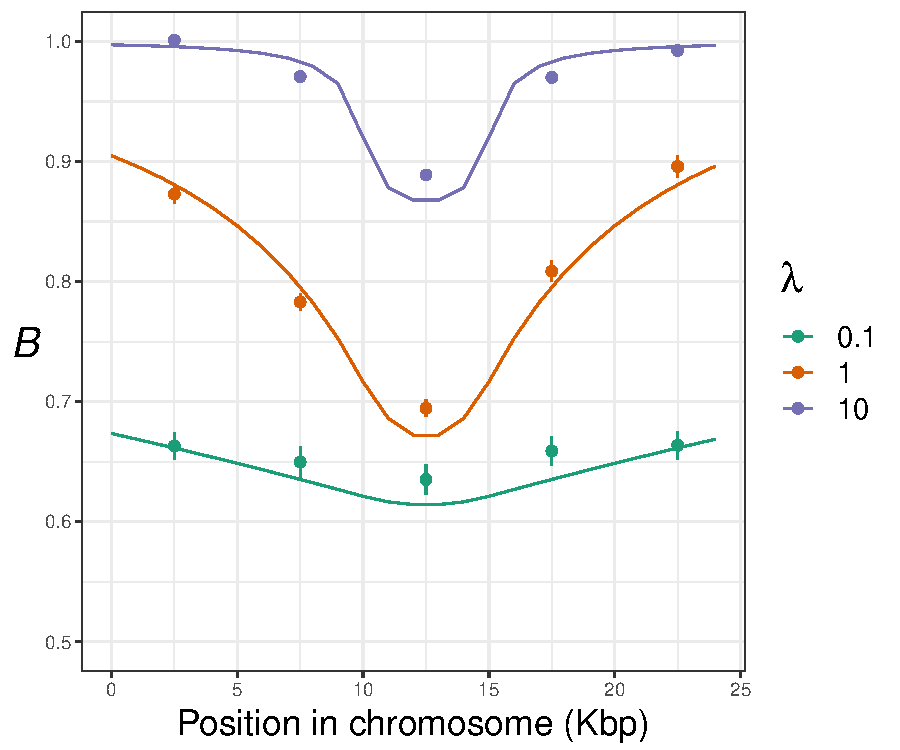
\includegraphics[width=0.7\textwidth]{../TheoreticalExpectation/B_fixed_plot}
\caption{The effects of background selection across simulated chromosomes. \textit{B} was calculated for simulated data by comparing observed $\pi$ to the neutral expectation of $4N_e\mu=0.01$. The lines show the theoretical expectation calculated using formulae from Nordborg et al (1996).}
\label{fig:BGS_fixed_plot}
\end{figure}

\end{document}


The first empirical evidence that selection at linked sites influences genetic variation across the genome came from studies in \textit{Drosophila}. Aguadé et al (1989) measured genetic variability in the \textit{yellow-achaete-scute} regions located at the tip of the X-chromosome. The \textit{yellow-achaete-scute} regions experience restricted crossing-over and Aguadé et al (1989) found that they harbour far less genetic variation than had been reported for more highly recombining regions of the genome. Aguadé et al (1989) suggested that selective sweeps (though that term was not coined until later), which reduce nucleotide diversity ($\pi$) to the greatest extent in regions of restricted recombination, potentially explained their findings. Begun and Aquadro (1992) then showed that there is a clear correlation between recombination rate and nucleotide diversity ($\pi$) using loci sampled from across the \textit{D. melanogaster} genome. Furthermore, Begun and Aquadro (1992) showed that there was little evidence for a correlation of between-species divergence and recombination rate, which one might expect if recombination were itself mutagenic. Soon afterwards, Charlesworth et al (1993) demonstrated that background selection could also potentially explain the correlation between $\pi$ and the recombination rate.  \\